\documentclass[a4paper]{article}

\usepackage{amsmath}
\usepackage{url}
\usepackage{acronym}
\usepackage[pdftex]{graphicx}


\acrodef{PDF}[PDF]{Probability Density Function}
\acrodef{GMM}[GMM]{Gaussian Mixture Model}
\acrodef{NB}[NB]{Naive Bayes}
\acrodef{kNN}[kNN]{k-Nearest Neighbour}

\begin{document}

\title{MLPM project \\ The effect of smoothness}
\author{Maarten van der Velden \\ 5743087 \\ \texttt{Maarten.vanderVelden@student.uva.nl} \and Carsten van Weelden \\ 0518824 \\ \texttt{cweelden@science.uva.nl}}
\maketitle

%\begin{abstract}
%\small \textit{ }
%\end{abstract}

\acresetall

\section{Introduction}
\label{sec:introduction}

In this paper we investigate the effect of smoothness of the dataset on the performance of classification algorithms. In order to investigate this we generate several artificial datasets of varying smoothness and look at the accuracy and loss of the resulting classifiers. In order to get insight into the effects we decompose the loss into its bias, variance, and noise components as defined in \cite{Domingos2000}.


To investigate the effect that smoothness has on classification performance we first need to define some idea of smoothness which we can easily vary and then run a set of experiments for different levels of smoothness. We view classification as a two class problem\footnote{As contrasted with a concept learning problem, in which there is one class which needs to be distinguished from the background.}, with each class being represented by some \ac{PDF} over the attribute space. Given this view the \emph{smoothness} of a class is determined by the shape of the \ac{PDF}. We define the \ac{PDF} for each class as a \ac{GMM} with $k$ mixture components. Intuitively, the smoothness is then determined by the number of components in the mixture. With just one component the \ac{PDF} corresponds to a Gaussian distribution which is very smooth, while increasing the number of components increases the peakedness of the distribution, making it less smooth.

One way to see this is in terms of inherent noise in the problem, which we define as the noise in definition 4 of \cite{Domingos2000}:
\begin{equation}
\label{eq:noise}
N(x) = E_t[L(t,y_*)]
\end{equation}
If we keep the standard deviation of the distributions approsimately equal, then with more components we will have a higher average probability that the \ac{PDF}s overlap for a datapoint $x$. Since the Bayes optimal prediction predicts the class for which the \ac{PDF} is highest at $x$, the noise is proportional to the area under the \ac{PDF} for which the \ac{PDF} of the other class is higher. In other words, the more components make up the distribution of a class, the more overlap there is between classes, and therefore the higher the noise component in the loss is.

To show this effect we generated \ac{GMM}s with an increasing amount of components and measured their noise. The models where generated according tot he method described in section \ref{sec:experimental_method}. Averaged over 25 random models of the same number of components, it is clear that the noise increases with the number of components, growing asymptotically towards 0.5, which represents the amount of noise where the Bayes optimal decision is correct half of the time: chance level. The results are shown in Figure \ref{fig:noisepercomp}.

\begin{figure}[H!]
    \centering
    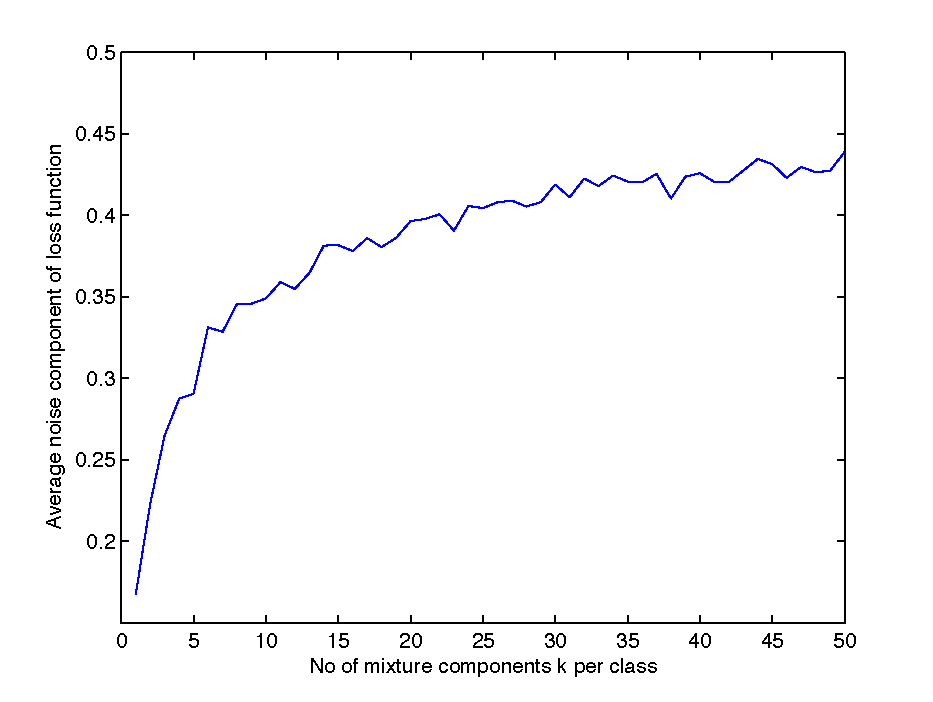
\includegraphics[width=0.9\textwidth]{noisePerK.pdf}
    \caption{The effect on the noise of the use of more mixture components in the \ac{GMM}. \label{fig:noisepercomp}}
\end{figure}

\section{Experimental method}
\label{sec:experimental_method}

To investigate the effect that the smoothness of the distributions has on classification performance we run a set of experiments. We generate a set of two-class problems with a given smoothness (as characterized by the number of components in the \ac{GMM} representing each class) and for each problem we estimate the expected loss, average bias, and average variance.

\begin{enumerate}
\item We generate a problem containing two classes denoted $C_0$ and $C_1$. Each class is represented by a \ac{PDF} which we define as a \ac{GMM} with $k$ components\footnote{We use a 2-dimensional attribute space for ease of visualization.}. We do this for $k = [1 .. 5]$. We pick the parameters corresponding to component $j$ of class $i$ as follows. The prior probability for each component is $\pi_{ij} = rand([1 .. 5]) / Z_i$ where $Z_i$ is a normalizing factor such that $\Sigma_{j} pi_{ij} = 1$. The mean of each component is $\mu_{ij} = (rand([-1,1]),rand([-1,1]))$. We use a scalar covariance matrix $\sigma I$ with $\sigma = rand([0.1,0.4])$.
\item For each two class problem we generate a set of 50 training sets $D = \{d_1, d_2, ..., d_{50}\}$ and a corresponding test set $T$. We do this for $|D| \in {10, 100, 1000, 1000}$ with half of the data points being sampled from each class. For the test set $|T| = 1000$, also with half of the points being sampled from each class.
\item We train a classifier on each training set $d \in D$ and evaluate the loss on the test set.
\item Finally, we compute the average bias and average variance on $T$ over all the training sets $d \in D$.
\end{enumerate}

We compute the loss as 0/1-loss and report the mean over all training sets and all problems for each number of mixture components and for each size of training set. We compute the average bias and average variance as given in \cite{Domingos2000} and again report the mean over all training sets and all problems given the number of components in each class and the training set size.

We perform these experiments with two different classifiers: \ac{NB} and \ac{kNN}. \ac{NB} does not have any parameters, so we simply train it once and calculate its predictions. For \ac{kNN} we have to select $k$, the number of neighbours. Since we are interested in the best \ac{kNN} classifier possible for each problem and training set, we perform an oracle run and select the $k$ which gives the best result on the test set. We do not try every value for $k$ but we sample 10 equidistant values from the range $[1 .. |D|]$, thus ranging from Nearest Neighbour classification to simply predicting the mean over the whole data.

For \ac{NB} we expect that for less smooth problems the expected loss will be higher, the intuition being that less smooth problems are harder to learn. For the same reason we expect the bias component of the loss to increase with the number of components per class. For both we expect them to be lower for larger training sets. For the average variance we expect to see that it increases with the amount of mixture components, but we expect this increase to be greater for smaller sizes of training set, since there are less datapoints per mixture component.

\section{Results}
\label{sec:results}

\subsection{Naive Bayes}
We trained Naive Bayes classifiers for all settings of the \ac{GMM} we defined in the last section. The resulting error is shown in Figure~\ref{fig:nbloss}, and the subdivision of this into bias and variance can be seen in Figures~\ref{fig:nbbias} and \ref{fig:nbvar} respectively.

\begin{figure}[H!]
    \centering
    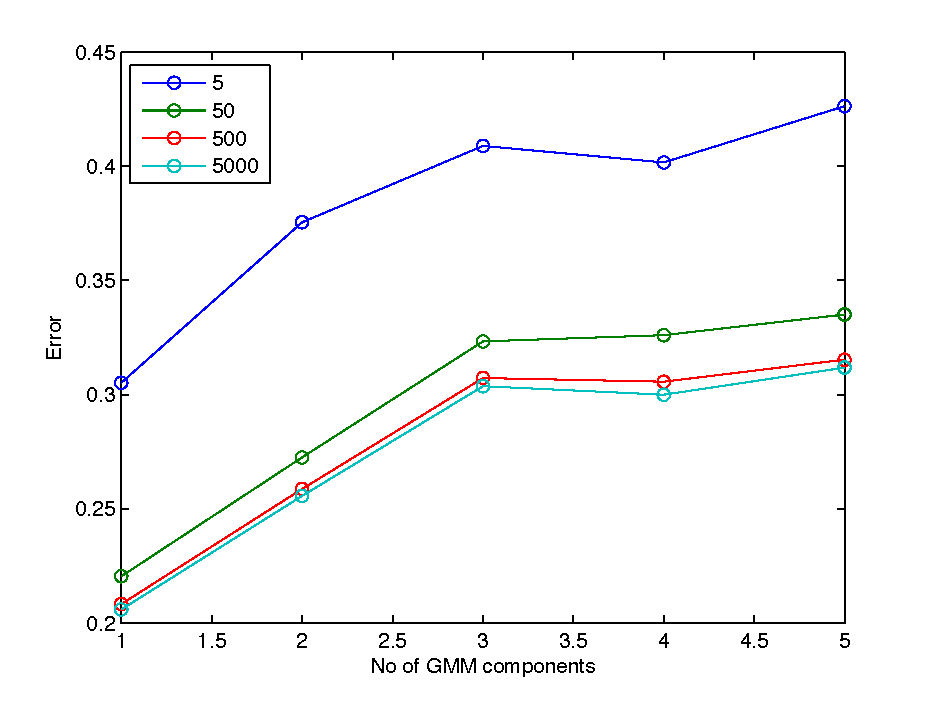
\includegraphics[width=0.8\textwidth]{nb_loss_1-5c.pdf}
    \caption{The average error of the Naive Bayes classifier on different amounts of training data, given different levels of smoothness of the data. \label{fig:nbloss}}
\end{figure}
\begin{figure}[H!]
    \centering
    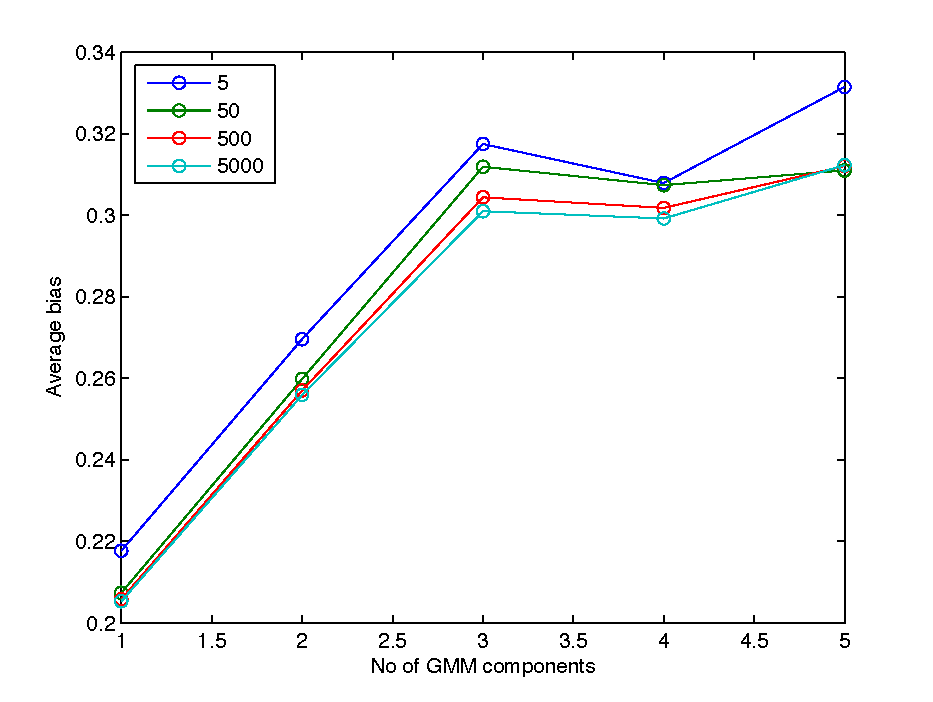
\includegraphics[width=0.8\textwidth]{nb_bias_1-5c.pdf}
    \caption{The average bias of the Naive Bayes classifier on different amounts of training data, given different levels of smoothness of the data. \label{fig:nbbias}}
\end{figure}
\begin{figure}[H!]
    \centering
    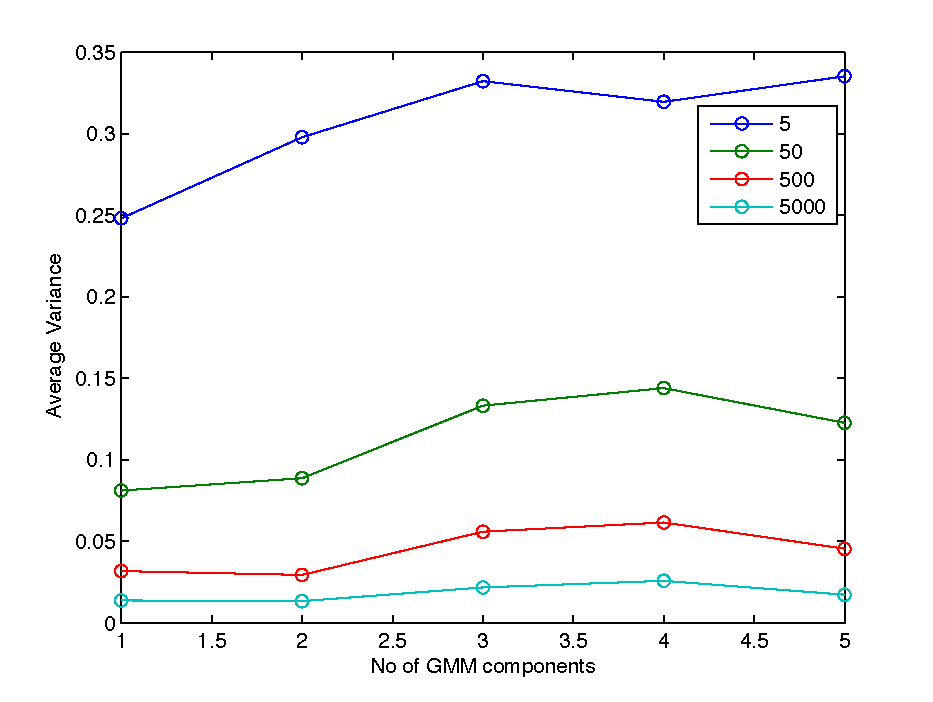
\includegraphics[width=0.8\textwidth]{nb_variance_1-5c.pdf}
    \caption{The average variance of the Naive Bayes classifier on different amounts of training data, given different levels of smoothness of the data. \label{fig:nbvar}}
\end{figure}

The figures show that in general, less training data results in a higher loss and variance, which was to be expected. Furthermore, the loss is higher when the smoothness increases. This might result solely from there being more noise, but Figure~\ref{fig:nbbias} shows that the bias increases sharply on less smooth data too.
There is less increase in the amount of variance overall, but this increase seems to be more significant with less training data than on much training data.
%Something on the dips in the variance? Wait for final results.

\subsection{kNN}


\section{Conclusion}



%Design choices:
% 2 class problem (2 PDFs) or concept learning problem (1 PDF versus rest). How to define the PDF (MVD, GMM, uniform)?
% Things to vary and try out: number of dimensions, real noise (next to the inherent noise), different number of components per class or number of datapoints per class, forms of PDF, learning algorithm (NB, kNN, ANN, Dec. Trees, SVM).

%Initial experiments:
% 2d 2 class
% GMM 1-5 mixtures (k) per class
% for each k:
%  m = |D| := 5 - 50 - 500 - 5000 (per class)
%  z = |T| := 1000 (500 per class)
% 100 runs each to estimate bias/variance/noise
% ?? runs each to average over different 2 class problems (e.g. pick new GMM each time)

%Workflow:
% 1. create pdfs: pick pi, mu, Sigma for each class {0,1} and k = 1-5
% 2. sample 100 datasets for each choice of k (= 400 total)
% 3. sample T
% 4. compute y_*
% 5. compute y_m = mode(t-y_*)
% 6. train classifier on each d \in D
% 7. evaluate on T
% Repeat enough times to get stable average over possible problems

%Measures:
% Accuracy: |TP|+|TN|/z
% Average bias E_x[L(y_*, y_m)]
% Average var E_x E_D[ L(y_m, y) ]
% Dataset noise L(t,y_*)

\end{document}
